\documentclass[UTF8,a4paper,zihao=-4,fontset=mac]{ctexart}
\usepackage[margin=2.5cm]{geometry}
\usepackage{amsmath,amssymb,amsthm,booktabs,array,graphicx,float,caption}
\usepackage{fontspec,xcolor,hyperref,fancyhdr,enumitem}
\setmainfont{Times New Roman}
\setlength{\parindent}{2em}
\setlength{\parskip}{0pt}
\linespread{1.18}
\setlist{nosep,leftmargin=2em}
\captionsetup{font=small,labelsep=quad}
\renewcommand{\topfraction}{0.9}
\renewcommand{\textfraction}{0.08}
\renewcommand{\floatpagefraction}{0.85}
\hypersetup{hidelinks}
\pagestyle{fancy}\fancyhf{}\fancyfoot[C]{\thepage}
\renewcommand{\headrulewidth}{0pt}
\newcommand{\pos}[1]{\left(#1\right)_+}
\newcommand{\E}{\mathbb E}
\newtheorem{proposition}{命题}
\title{基于跨日因果仿射规划与条件 Markov 价值反馈的微网经济调控}
\author{}\date{}

\begin{document}
\maketitle
\vspace{-2.4em}
\begin{abstract}
\IfFileExists{generated/abstract.tex}{\input{generated/abstract.tex}}{本文正在完成冻结参数后的全年闭环评价。本稿为内部方法排版稿，年度费用、区间与采用结论尚未填入，不作为完成稿交付。}
\par\noindent\textbf{关键词：}跨日储能；因果仿射决策；条件联合场景；凸动态规划；滚动时域
\end{abstract}
\clearpage

\section{问题重述}
微网同时面对不可任意转移的用电需求、具有预测误差的光伏出力以及可跨时段储能的电池。购电计划具有提前承诺和受限调整的特点，偏差通过紧急购电与弃电消化。因此，电池价值不只来自同一天的峰谷价差，还来自库存对未来净需求及合同偏差的缓冲。

问题一在给定单日需求与光伏条件下确定购电及充放电计划，建立可独立核算的确定性基准。问题二在负荷和光伏逐时实现、原始日合同不能调整的条件下安排提前购电并实时调节电池。问题三利用合法发布的光伏预报和日内合同修改机会降低偏差代价。问题四在浮动电价下分别延续问题二、三的合同权限，处理净需求与价格误差的共同变化。

本文采用两层滚动框架：上层在合同发布节点优化共同承诺和可因果调整的未来计划，下层在每个时段根据当前净需求与库存作出可行的电池动作。所有问题采用同一物理模型和结算器。问题二至四的主评价为 2025 年 2 月 1 日至 12 月 31 日的 334 日连续回放；一月用于暖启动与参数开发。正式回放的时间原点对应 2 月 1 日零时，初始库存按共同设置取 6000 kWh，不要求它由一月开发轨迹自然继承。真实年末库存同为 6000 kWh，日界处不重置库存。

\begin{figure}[!t]\centering
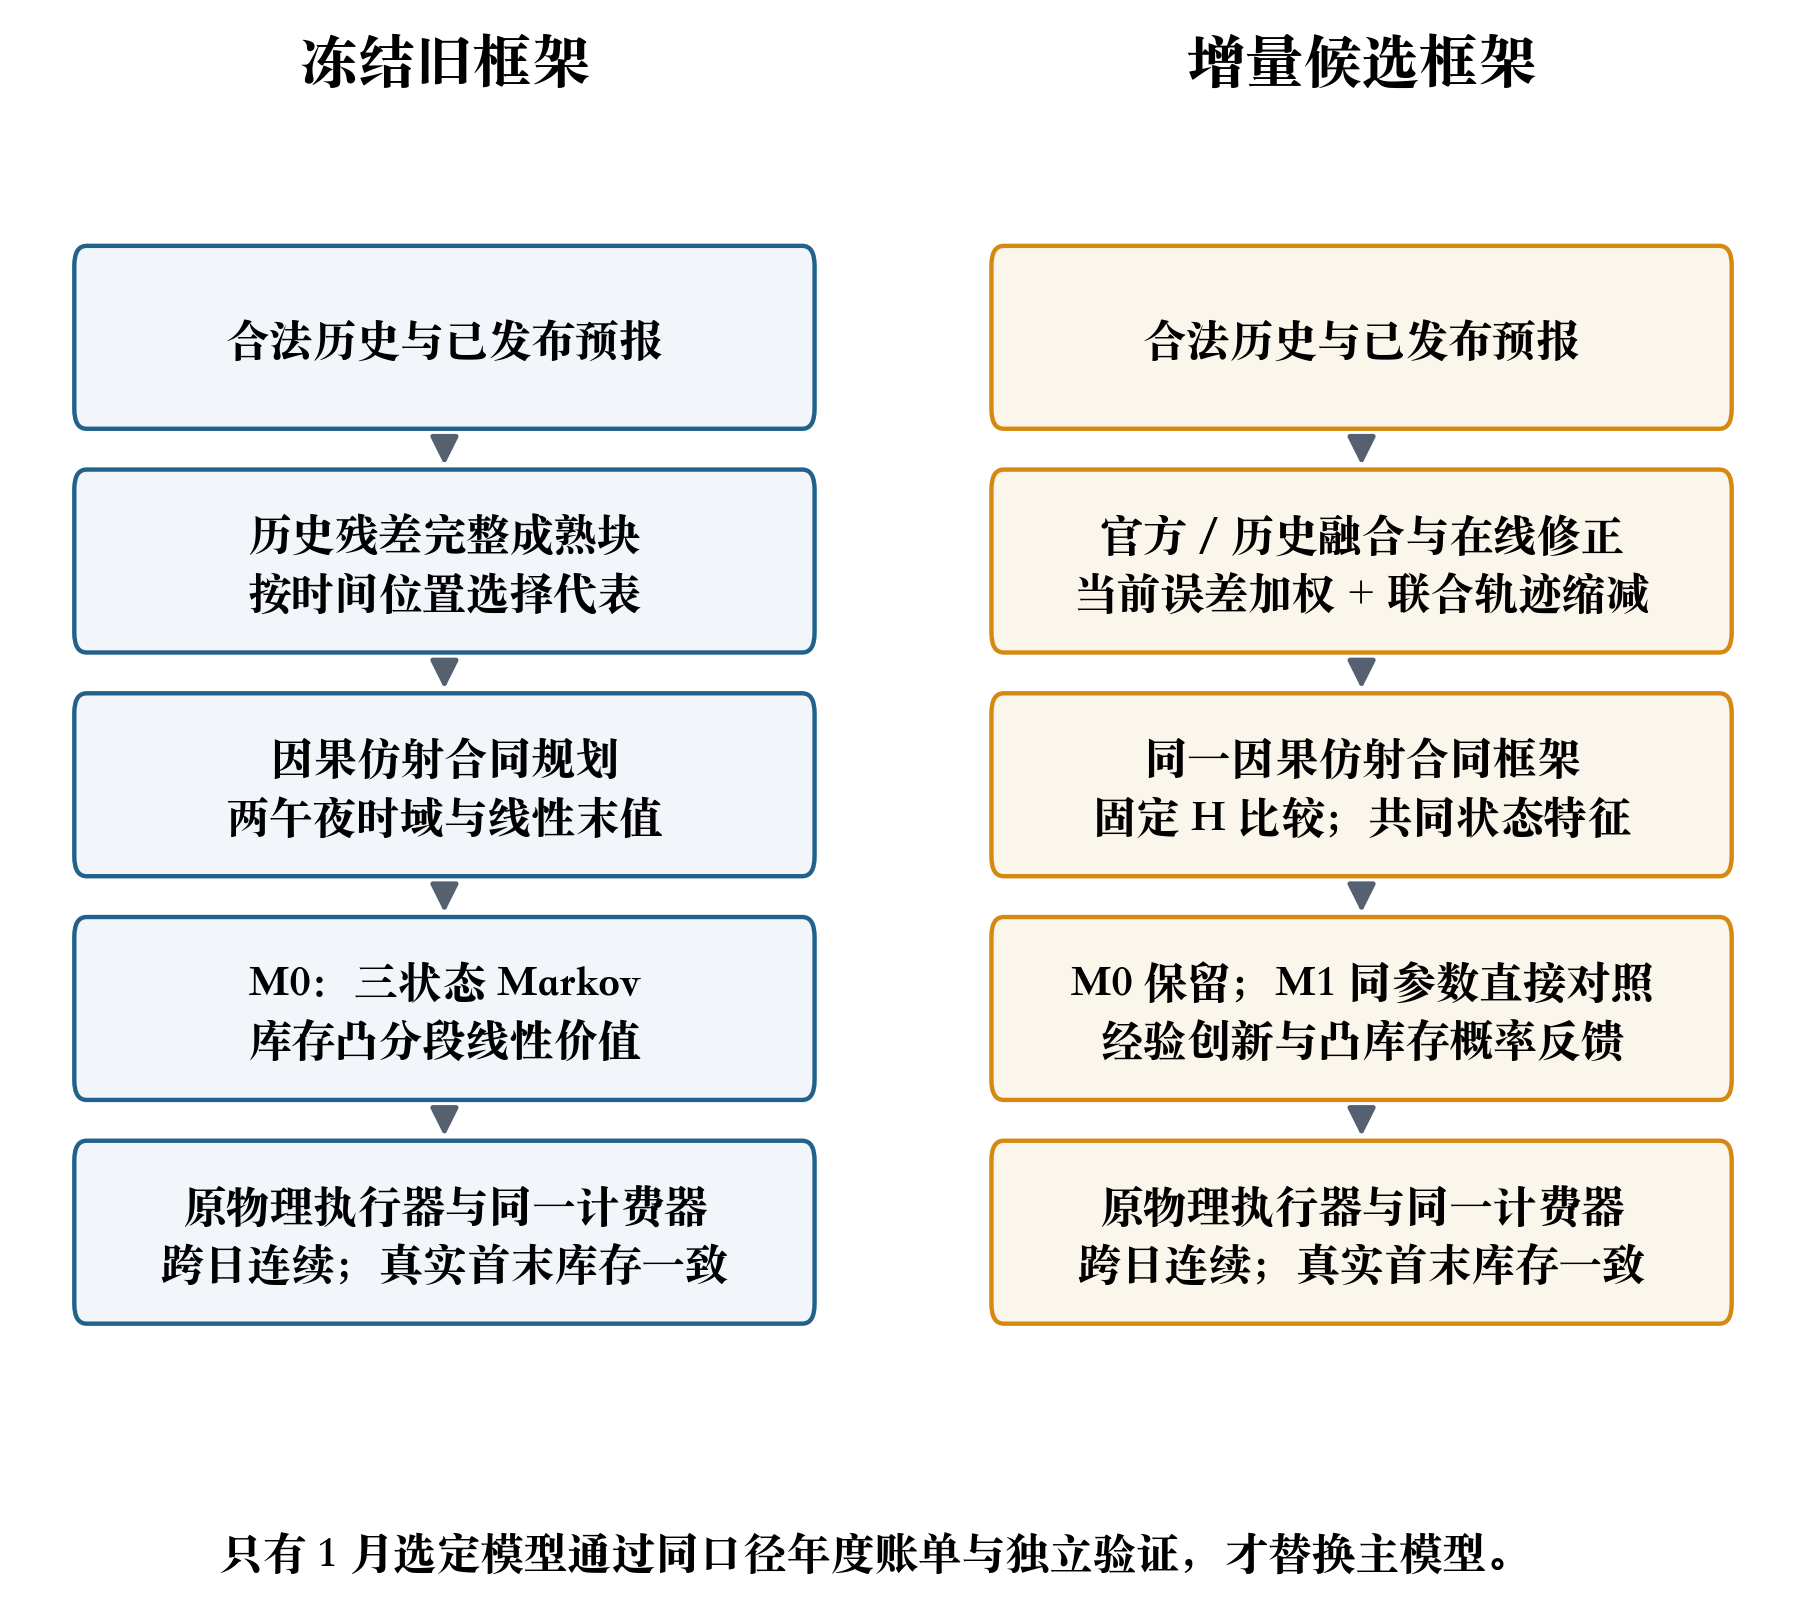
\includegraphics[width=.95\linewidth]{../figures/新旧模型结构.png}
\caption{原框架与增量候选共享物理执行和计费层，新增模块通过同口径闭环证据决定是否采用。}
\end{figure}

\section{假设、信息结构与符号}
\subsection{假设及适用范围}
保留题面给出的容量、功率和充放电效率，不在主结果中加入题面未给出的退化、自放电或并网容量参数。紧急购电和弃电按题面的权限处理。减少合同量沿用冻结基线的净额解释，即原价退还并支付半价违约金，净抵扣半价；所有比较始终使用同一解释。

浮动价格附件未给出真实披露时间戳。为保持信息权限与基线一致，假设上一已结束时段的结算价格可见，当期价格在电池动作后披露。该假设限定了问题四的结论范围，不等同于价格在实际市场中的唯一披露制度。已发布光伏预报仅在其覆盖范围内使用；尚未发布的更新不能提前进入计划。

历史残差用于构造当前条件下的有限经验分布。本文不假设全年误差独立同分布，也不把有限代表场景等同于真实随机规律。模型输出的全年账单是冻结策略在该年份、该信息结构下的闭环结果。

\subsection{统一符号与可用信息}
\begin{table}[H]\centering\caption{主要符号及单位}
\begin{tabular}{lll}\toprule
符号&含义&单位\\\midrule
\(L_t,P_t,n_t\)&负荷功率、光伏功率、时段净需求&kW、kW、kWh\\
\(q_t,r_t\)&原始合同、最终有效合同电量&kWh\\
\(c_t,d_t,e_t,s_t\)&充电、放电、紧急购电、弃电&kWh\\
\(E_t\)&时段开始库存&kWh\\
\(p_t\)&固定或实际结算电价&元/kWh\\
\(a,H,T_\star\)&规划原点、时域小时数、真实评价终点&时段、小时、时段\\
\(\omega_s,x_t,V_t\)&场景概率、可观测误差状态、库存值函数&--\\
\bottomrule\end{tabular}
\end{table}

令 \(\mathcal F_t^-\) 为时段交付前、合同发布时已知的信息，包含截至上一时段的实际观测和当前已发布预报；电池动作信息为
\begin{equation}
\mathcal F_t=\mathcal F_t^-\vee\sigma(n_t).
\end{equation}
根合同及当次调整对 \(\mathcal F_t^-\) 可测，电池动作对 \(\mathcal F_t\) 可测。问题四的当期实际价格不属于这两个动作的信息集。代码严格按合同发布、当前净需求观测、电池执行、当前价格披露的顺序推进。

\section{统一物理模型与跨日库存价值}
时段长为 10 分钟，功率转化为电量后有
\begin{align}
n_t&=(L_t-P_t)/6,\\
r_t+e_t+d_t-c_t-s_t&=n_t,\\
E_{t+1}&=E_t+\eta c_t-d_t/\eta,\qquad \eta=0.9,\\
1200\le E_t&\le10800,\qquad 0\le c_t,d_t\le 5000/6.
\end{align}
同时要求 \(q_t,r_t,e_t,s_t\ge0\)。记时段充放电量上限为 \(M=5000/6\)。
实际执行保证不同时充放电。统一账单为
\begin{equation}\label{eq:bill}
J=\sum_t p_t\bigl[q_t+1.5\pos{r_t-q_t}-0.5\pos{q_t-r_t}+5e_t\bigr]
=\sum_t p_t\bigl[r_t+0.5|r_t-q_t|+5e_t\bigr].
\end{equation}
问题二及问题四的对应设置要求 \(r_t=q_t\)。允许调整时，首六小时仍执行原合同，后续只在合法发布节点修改未交付部分。

\begin{proposition}
令库存增量为 \(\Delta=E_{t+1}-E_t\)，满足 \(-M/\eta\le\Delta\le\eta M\) 及下一库存边界。在价格非负、免费弃电且不加入循环奖励的口径下，实现该增量可以选取不同时充放电的动作，母线侧净耗电为
\begin{equation}\label{eq:g}
g(\Delta)=\max\{\eta\Delta,\Delta/\eta\}.
\end{equation}
给定合同及库存增量，最少紧急购电为 \(\pos{n_t-r_t+g(\Delta)}\)。
\end{proposition}
\begin{proof}
当 \(\Delta\ge0\) 时取 \(c=\Delta/\eta,d=0\)；当 \(\Delta<0\) 时取 \(c=0,d=-\eta\Delta\)。同时增加充放电只额外消耗能量，允许弃电时可将这种消耗替换为弃电而不增加费用。母线不足部分用紧急购电补齐，剩余部分弃电，即得结论。
\end{proof}

式\eqref{eq:g}及账单中的绝对值均可用线性上图约束表示。问题一据此形成单日确定性线性规划，要求 \(E_0=E_{144}=6000\)，并由显式充放电量、库存和逐时费用独立验证。对问题二至四，连续跨日条件为
\begin{equation}
E_{d+1,0}=E_{d,144},\qquad E_0=E_{T_\star}=6000.
\end{equation}
这一设置避免了每日强制闭合导致的库存价值截断，也避免自由年末消耗库存带来的不公平收益。真正终点进入窗口时，上层施加硬约束；物理执行器同时维持剩余时段到终点的可达性。

\section{合法预测、条件联合场景与缩减}
\subsection{官方预报和历史预测融合}
历史预测模型族由一月选定。对于允许官方光伏预报的设置，在其覆盖范围内采用
\begin{equation}
\widehat P_{a,t}=\beta\pos{\widehat P^{\mathrm{off}}_{a,t}+\gamma\bar e_a^{\mathrm{off}}e^{-(t-a)/36}}
+(1-\beta)\widehat P^{\mathrm{hist}}_{a,t}.
\end{equation}
在线误差均值只使用最近 36 个已实现时段及当时已经发布的原始官方预报。历史模型保留原有的已观测误差修正；官方覆盖范围外回到历史预测。融合权重和修正增益先按一月下一六小时光伏误差选择，再由一月闭环账单检验模块价值。未来预报更新只在实际发布后使用。

\subsection{完整成熟历史轨迹}
规划长度为 \(T\) 个时段时，历史残差块的起点 \(h\) 必须满足
\begin{equation}
\mathcal H_a=\{h:h+T\le a,\ h\equiv a\pmod{144}\}.
\end{equation}
从满足暖启动要求的候选中取最近至多 \(W\) 个。历史预测在各自原点重建；块内最后目标未实现时，整块都不能使用。这个限制也在缓存读取前执行。

以短期净需求误差和持续状态构造当前条件向量；浮动电价时同时加入已披露价格误差及持续状态。历史起点采用相同定义。标准化距离得到条件质量
\begin{equation}
\omega_h(a)\propto\exp\left[-\frac{\|D_a^{-1}(u_h-u_a)\|^2}{2b_a^2}\right],\qquad
\sum_{h\in\mathcal H_a}\omega_h(a)=1.
\end{equation}
尺度和带宽仅由合法候选估计。该构造以可观测协变量调整经验决策分布，借鉴条件加权处方的思想\cite{bertsimas}，不套用其与本题采样条件不符的一致性结论。问题四将净需求和价格残差按完整同一历史块保留，不独立拆分其相关性。

\subsection{代表轨迹与覆盖诊断}
对标准化后的完整联合轨迹计算距离，用加权前向选择及有限轮 PAM 交换选择代表，再把候选概率转移给最近代表。对应近似目标为
\begin{equation}
\min_{\mathcal S\subseteq\mathcal H_a,\ |\mathcal S|\le S}
\sum_{h\in\mathcal H_a}\omega_h(a)\min_{s\in\mathcal S}d(h,s).
\end{equation}
不声称离散代表选择达到全局最优。记录实际候选数、代表数、权重有效样本量、输运距离和尾部保留率。一月历史不足时，较大的请求窗口未必带来更多样本；这种不可区分性必须如实报告。

\section{因果仿射合同规划}
未来原合同与修改合同分别在其信息截止节点使用状态特征：
\begin{align}
q_t^s&=\bar q_t+K_{d(t)}^q\phi_{\rho_q(t)}^s,\\
r_t^s&=\bar r_t+K_{b(t)}^r\phi_{\rho_r(t)}^s.
\end{align}
合同特征只包含发布节点前已知的信息；相同历史前缀产生相同合同。库存反馈允许使用当前净需求，浮动价格反馈只使用上一已结束时段的误差。采用受限仿射决策规则\cite{bental}使有限场景规划保持可解，但本文的经验期望费用模型不继承全扰动鲁棒可行性的保证。

上层以代表概率加权式\eqref{eq:bill}，并加入库存末值，在每条代表路径上约束容量、功率和合同权限。已形成的当日原合同保持不变。样本外实际动作由同一执行器保证可行。

固定时域在非午夜结束时仍有同日原合同未覆盖的后缀。本文显式补充零反馈、等于当前原点非负净需求预测的合同后缀，并记录信息截止时刻。后缀交付费用未纳入核心目标，因此其末值是库存截断近似，不能解释为包含完整合同状态的精确继续价值。

\section{凸 Markov 实时价值反馈}
\subsection{基线 M0}
保留三分位离散 Markov 状态和库存上的凸分段线性值函数。非均匀代表概率用于分位点、条件均价和转移统计；均匀三状态配置直接复用原控制器。加权版本的转移伪计数为 \(S\omega_s\)，因此代表数量变化也会影响平滑强度，该因素与场景几何变化共同构成 S 敏感性的解释范围。

记当前净需求分位组为 \(k\)，组内场景集合为 \(\mathcal C_{t,k}\)，归一化组内概率为 \(\omega_{s\mid k}\)，组内条件均价为 \(\bar p_{t,k}\)，带平滑的组间转移概率为 \(P_{t,k\ell}\)。空组仅在当期净需求分布和均价上回退到完整场景；转移空行仍按伪计数平滑为下一各组的均匀概率。定义下一库存的条件继续费用
\begin{equation}
F_{t,k}(E')=\sum_\ell P_{t,k\ell}V_{t+1,\ell}(E').
\end{equation}
在库存网格节点按下式反向递推，再作凸弦插值：
\begin{equation}
V_{t,k}(E)=\sum_{s\in\mathcal C_{t,k}}\omega_{s\mid k}
\min_{E'\in\mathcal E(E)}\left\{5\bar p_{t,k}\pos{n_t^s-r_t+g(E'-E)}+F_{t,k}(E')\right\}.
\end{equation}
物理库存域 \(\mathcal E(E)\) 由容量及单时段功率限制给出。在线已观测当前净需求后，定位其分位组，并将相同最小化式中的场景净需求替换为实际净需求。条件均价与分位转移是 M0 的统计近似；不把这种粗分组等同于完整可观测状态的充分统计量。合同常数费用从电池子问题省略，在实际结算中完整保留。

\subsection{增强状态候选及采用原则}
M1 将当前净需求误差、持续状态及已披露价格误差纳入连续外生状态，按六小时时钟段拟合经验创新模型，并以非负概率核连接有限支持点。库存仍保持一维凸分段线性结构；下层支持点递推与在线动作使用同一条件均价和转移核。具体算子、状态投影近似与执行器终点可达域见附录\ref{app:m1}。

该候选回答“在相同上层合同模型、场景构造和末值设置下，更换下层反馈是否改善闭环结果”的问题。它不自动替代三状态 M0，必须通过最终末值下的直接匹配对照，且开发期与全年回放均满足预注册采用门槛。不同反馈产生的库存会影响后续合同，因此匹配的是规划规则与信息权限，不要求两条闭环合同轨迹始终相同。

\subsection{末值和算法采用边界}
线性末值为 \(-\lambda E\)，基础系数取当前场景最后最多二十四小时价格的加权 25\% 分位数除以效率。比较零末值及合理倍率。下层真实终点采用有限罚 \(1000|E-6000|\)，硬终点可行性由上层和执行器保证，不能将有限罚写成无穷指示函数。

已有 SDDP 仅在共同两午夜接口下作为辅助末值对照；其库存切平面不能直接接到非午夜、尚携带未交付合同的边界。完美信息全时域 LP 作为乐观参照，但其与实际账单的差距同时包含信息和模型近似价值。信息松弛下界要求对目标随机律满足对偶可行性\cite{brown}；单年路径不能识别该真实随机律。未建立同分布、同信息的因果下界时不报告伪造的因果 gap。

\section{同口径闭环实验与结果}
预测模型族与超参数仅在一月开发，随后绑定程序、数据、预测配置和协议哈希冻结。正式区间按同一冻结估计规则，用已实现历史更新条件经验分布和回归系数；实际账单不参与这些统计更新或参数选择。时域比较为固定 48、72、96 小时；旧两午夜窗口单列，因为其日内前瞻依次为 48、42、36、30 小时。每个时域使用满足自身长度要求的成熟块，不能把历史集合及末值取值窗口变化全部解释为物理前瞻效应。

对各配置运行 334 日顺序闭环，逐时重算费用并形成逐日配对差。7 日移动块 bootstrap 采用共同日期索引、10000 次重采样，保留各问间同日相关性，报告全年节省的百分位 95\% 区间。依赖数据的块重采样思想见\cite{kunsch}；本文单年季节性资料并不自动满足平稳总体假设，区间仅作为该年稳定性诊断。

M1 在最终末值配置下与仅下层不同的 M0 直接比较。全年只检验一月选定挑战模型，不能从全年消融表另挑赢家。改善很小、只集中在局部日期或增加复杂度而缺少明确贡献的模块不进入主模型。

\IfFileExists{generated/results.tex}{\input{generated/results.tex}}{\par\noindent\textbf{内部排版稿提示：}完整年度结果、配对区间与采用结论尚待计算及独立验证。}

\section{验证与讨论}
独立验证覆盖母线平衡、库存递推、容量及功率边界、单向充放、午夜连续性、真实终点、合同发布权限、费用逐时重算和文件读回一致性。信息扰动检查固定合法历史，修改信息截止点之后的真实负荷、光伏、价格及未发布预报，先前形成的合同必须不变；固定当前净需求时，当前电池动作也不能被隐藏价格扰动改变。

小型显式充放电 LP 与上层凸表达及下层 Bellman 算子进行独立对照。该验证证明实现与所声明的近似模型一致，不把有限场景可行性、近似值函数或辅助 SDDP 收敛提升为原问题全局最优性。未被主模型采用的模块仍保留同口径结果，作为复杂度选择的证据。

\IfFileExists{generated/discussion.tex}{\input{generated/discussion.tex}}{}

\begin{thebibliography}{9}
\bibitem{bertsimas}Bertsimas D, Kallus N. From Predictive to Prescriptive Analytics[J]. Management Science, 2020, 66(3): 1025--1044.
\bibitem{bental}Ben-Tal A, Goryashko A, Guslitzer E, et al. Adjustable robust solutions of uncertain linear programs[J]. Mathematical Programming, 2004, 99(2): 351--376.
\bibitem{brown}Brown D B, Smith J E, Sun P. Information Relaxations and Duality in Stochastic Dynamic Programs[J]. Operations Research, 2010, 58(4-part-1): 785--801.
\bibitem{kunsch}Künsch H R. The Jackknife and the Bootstrap for General Stationary Observations[J]. The Annals of Statistics, 1989, 17(3): 1217--1241.
\end{thebibliography}

\appendix
\section{误差状态与合同信息截止的实现定义}
在当前规划原点固定预测参照，对 \(t\ge a\) 的块内误差及持续状态定义为
\begin{align}
\epsilon_{n,t}^{a}&=n_t-\widehat n_{a,t},&
z_{n,t}^{a}&=(1-\alpha)z_{n,t-1}^{a}+\alpha\epsilon_{n,t}^{a},\\
\epsilon_{p,t}^{a}&=p_t-\widehat p_{a,t},&
z_{p,t}^{a}&=(1-\alpha)z_{p,t-1}^{a}+\alpha\epsilon_{p,t}^{a}.
\end{align}
未来式中的实际量在规划中由同一成熟历史块的残差替代；上述定义不授权读取未来真实值。每次重新规划，持续状态以截至上一时段的短预测误差账本初始化。账本采用前一日同一时段作为短预测，即
\begin{equation}
\delta_{n,t}=n_t-n_{t-144},\qquad \delta_{p,t}=p_t-p_{t-144}.
\end{equation}
其指数平滑值从首个合法误差初始化，之后只顺序使用已实现项。当前条件向量为上一时段的两类误差及其平滑值；固定电价时只保留净需求两维。块内递推的两个初始平滑值取账本上一时段值，初始滞后价格误差明确取 \(\epsilon_{p,a-1}^{a}:=\delta_{p,a-1}\)。当前全部场景共用这一种子；历史起点则使用各自上一时段的账本值。因此，条件加权的原点状态与块内相对固定原点预测的状态参照有区别，两者通过上述初始化规则衔接。

统一状态上层在未来发布节点使用其前一已结束时段的特征。记该前一时段为 \(v=\rho-1\)，则原始特征为
\begin{equation}
f_v^s=(\epsilon_{n,v}^{a,s},z_{n,v}^{a,s},c_p\epsilon_{p,v}^{a,s},c_p z_{p,v}^{a,s}),
\qquad c_p=\sigma_n/\sigma_p,
\end{equation}
并使用加权中心化特征
\begin{equation}
\phi_\rho^s=f_{\rho-1}^s-\sum_k\omega_k f_{\rho-1}^k.
\end{equation}
标准差由未缩减的合法历史净需求、价格残差估计，并设置数值正下限。固定电价删除后两维。发布节点不晚于当前原点时，未来反馈项为零。已签原始合同直接固定；当前发布节点的原合同或允许调整的有效合同作为所有场景的共同决策优化。原合同的发布节点为交付日零时，允许修改的有效合同使用所在六小时时钟段的发布节点：
\begin{equation}
\rho_q(t)=144\lfloor t/144\rfloor,\qquad
\rho_r(t)=36\lfloor t/36\rfloor.
\end{equation}
首六小时或不允许修改的任务另施加有效合同等于原合同。库存反馈在当前净需求观测后执行，价格特征仍滞后一时段；因此它与下一合同发布时可用的价格特征相差一个披露节点。

增强状态的联合回归目标为
\begin{equation}
y_t=(\epsilon_{n,t+1}^{a},\epsilon_{p,t}^{a}),\qquad
\xi_{t+1}=y_t-(C_\tau x_t+d_\tau).
\end{equation}
联合创新同时连接下一净需求误差与当期尚未披露的价格误差。固定电价只保留第一维。持续状态的两行由同一误差创新按指数平滑恒等式生成，随后进行价格正值截断及相应状态重建；正文的线性状态式仅表示截断前提议。

\section{增强状态反馈的近似 Bellman 模型}\label{app:m1}
动作状态取 \(x_t=(\epsilon_{n,t},z_{n,t})\)，浮动电价时扩展为
\begin{equation}
x_t=(\epsilon_{n,t},z_{n,t},\epsilon_{p,t-1},z_{p,t-1}).
\end{equation}
在每个滚动原点固定预测参照，按六小时时钟段共享回归：
\begin{equation}
x_{t+1}^{\mathrm{raw}}=A_\tau x_t+b_\tau+B\xi_{t+1}.
\end{equation}
仅拟合净需求误差和隐藏价格误差，EMA 行按 \(z'=(1-\alpha)z+\alpha\epsilon'\) 构造。创新为成熟历史的联合回归残差，采用实际残差代表，不强制高斯。价格截断为正后重建价格误差和 EMA。每六小时重规划时统计状态重新定位，库存不重置；不声称该有限状态严格充分。

外生状态使用路径支持点和非负核，库存仍使用一维凸分段线性结构。令 \(w_{t,s}(x)\) 为归一化插值权重，\(\mu_i\) 为经验创新概率，近似转移为
\begin{equation}
\widetilde P_t(x,k)=\sum_s w_{t,s}(x)\sum_i\mu_i
w_{t+1,k}\bigl(T_\tau(x_{t,s},\xi_i)\bigr).
\end{equation}
同一当前状态核也用于混合截断后的条件均价 \(\bar p_t(x)\)。在库存网格节点进行
\begin{equation}\label{eq:bellman}
V_t(E,x_{t,s})=\min_{E'\in\mathcal E(E)}\left\{
5\bar p_t(x_{t,s})\pos{n_{t,s}-r_t+g(E'-E)}
+\sum_k\widetilde P_t(x_{t,s},k)V_{t+1}(E',x_{t+1,k})\right\}.
\end{equation}
其中物理动作域为
\begin{equation}
\mathcal E(E)=[\max\{1200,E-M/\eta\},\min\{10800,E+\eta M\}].
\end{equation}
连续库存使用弦插值。在线动作以实际已观测净需求替换支持点净需求，并使用与式\eqref{eq:bellman}相同的概率核与均价。当前价格先取条件期望，再选择动作。合同固定后的当期常数费用可在电池子问题中省略，但最终账单仍完整核算。

执行器还将动作投影到真正终点的可达区间。若动作后剩余 \(R=T_\star-t-1\) 个时段，则实际采用的库存域为
\begin{equation}
\mathcal E_t^{\mathrm{exec}}(E)=\mathcal E(E)\cap[6000-R\eta M,\ 6000+RM/\eta].
\end{equation}
该额外约束属于全局执行安全层，不应与下层有限罚值递推的物理动作域混写。

非负概率混合保持库存凸性，避免高维密集网格。支持点投影会近似外生状态演化；投影标签不逐条满足原 EMA 递推。下层采用上层未来合同的名义路径，未把所有未来合同适应性纳入 Bellman。因此 M1 是可解释、可验证的近似反馈，不是原随机控制问题的全局解。

\section{程序与结果对应关系}
\begin{table}[H]\centering\small\caption{可复现程序的职责}
\begin{tabular}{p{6.2cm}p{8cm}}\toprule
文件&对应内容\\\midrule
\texttt{nextgen\_scenarios.py}&合法预测、完整成熟残差块、条件权重与轨迹缩减\\
\texttt{nextgen\_control.py}&因果仿射 LP、离散及增强 Markov 凸反馈\\
\texttt{nextgen\_run.py}&顺序回放、原执行器、逐时账单与库存\\
\texttt{run\_incremental\_experiments.py}&一月阶段开发与正式配置冻结\\
\texttt{compare\_incremental\_results.py}&逐日配对费用、块 bootstrap、消融汇总\\
\texttt{evaluate\_adoption.py}&单一冻结挑战模型及 M1 直接贡献门槛\\
\texttt{review/}&独立信息、数学、物理、计费和代码检查\\\bottomrule
\end{tabular}\end{table}
\IfFileExists{generated/appendix.tex}{\input{generated/appendix.tex}}{}
\end{document}
